\chapter{实例抽取}
对于一项活动,除了
\section{标注规则}
为了验证标注的有效性,我们

\section{活动类别抽取}
\subsection{简单规则匹配}
\subsection{引入句法分析}
对错误结果的分析发现,大约有12\%的错误分类是因为活动表述的语法结构比较复杂,简单的规则匹配无法正确识别句子的主干。一种情况是,活动以主谓结构出现,如``麻辣烫真是太好吃了'',应该提取出``吃麻辣烫'';还有一种情况是动宾结构比较复杂,无法匹配比如``陪父母看了一场周星驰拍的很有意思的电影'',应该抽取出``陪父母''和``看电影''。为了正确处理这些情况,我们需要对句子进行句法分析,组织成依存树。

Stanford Parser(http://nlp.stanford.edu/software/lex-parser.shtml)是斯坦福大学自然语言处理组开发的句法分析工具。它主要提供英语语言的解析,但是也提供中文、德语、阿拉伯语等多语种的解析,但它的处理结果并不非常直观。最终本文选择哈尔滨工业大学开源的语言技术平台(Language Technology Platform, LTP)\cite{che2010ltp}作为句法分析工具。LTP提供分词、词性标注、命名实体识别、依存句法分析、语义角色标注等功能,提供自然语言处理的集成解决方案。

\begin{figure}[!h]
\centering
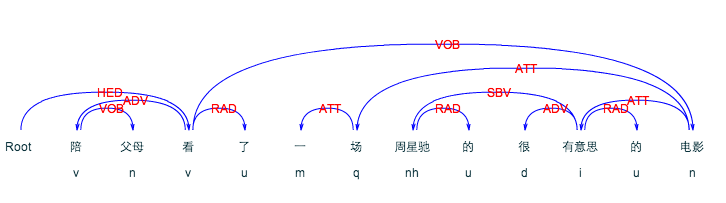
\includegraphics[width=0.9\textwidth]{ltpdemo1.png}
\caption{LTP句法分析结果}
\label{fig:ltp_demo}
\end{figure}


\subsection{局限}

\section{地点抽取}
我们与搜狐合作,得到的国内主要城市的兴趣点(POI, point of interest)数据,来辅助我们的地点抽取。POI数据中包含位置,类型,名称等信息,样例如表\ref{table:poi_sample}。
\begin{table}[!h]
\centering
\begin{tabular}{|c|c|}
\hline
{\heiti Attribute} & {\heiti Value} \\
\hline
Name & 北京密云东方商贸大厦 \\
\hline
Address & 北京市密云县新东路40 \\   
\hline
Contact & 010-69043424    \\
\hline
Type & 购物场所        \\
\hline
Category & 一般商场      \\  
\hline
Province & 北京市  \\
\hline
City & 北京市  \\
\hline
District & 密云县 \\  
\hline
Longtitude &13008155.004543  \\
\hline
Latitude & 4892797.007317 \\
\hline
\end{tabular}
\caption{POI样例}
\label{table:poi_sample}
\end{table}

\section{情感极性分析}
在活动抽取中,如果微博中包含用户参与的一项活动,我们希望了解用户参与这项活动时的心情状态如何,帮助我们发现活动本身是正面还是负面,这样帮助推荐系统进行选择。因此,需要获取微博的情感极性。

\subsection{方法概述}
本文的工作中,对微博进行三分类,正面(positive),中性(neutral)和负面(negative)。

我们对非监督和监督学习均进行了尝试。在非监督的方法中,我们从知网(Hownet)等途径获取了中文的情感词典,共有4986个积极词汇和4818个消极词汇,包含动词、形容词和名词。对每一条微博,我们首先计算计算其中积极、消极词汇的数量$n_pos$和$n_neg$,若其差值$|n_pos-n_neg|<\theta$,则认为微博是中性的,否则判别为词数多的类别。但这样简单的非监督方法只能达到55\%的正确率(注意到这是三分类问题,这个结果还是比随机分类(33\%)和全部判为最多的类别(45\%)要好很多的)。为此,我们使用监督学习的方法,使用以下特征训练分类器

\begin{enumerate}
\item Bigrams和Unigrams的频度。使用bigram的原因是,情感词之前常常会带有修饰性的前缀,如``不'',``非常'',有时会加强或者逆转情感词的极性。因此对于较频繁出现的模式,是哟高bigram作为特征。
\item 正面词、负面词的频度。这可以根据情感词典和
\item 表情符号。用户在发布微博时,常常会加入一些表情,如``高兴'',``愤怒'',有时用户选择表情并不关心这个表情具体的含义是什么,但是也可以体现出用户当时的心理状态。
\end{enumerate}
同时,为了加快训练速度和减少噪声,我们将过于稀疏,即出现次数少于一个下界的特征滤除。

\subsection{实验结果与分析}

我们标注了20829条包含活动信息的微博,根据其情感极性标注为5级,-2为很负面,-1为一般负面,0为中性,1为一般积极,2为很积极,其中分级-2、-1为负面,+1,+2为中性,0为中性。为了避免不同人倾向性的不同,每条微博会有至少两个人标注,如果出现分歧,由实验者最终决定类别。在数据中,共有9462条为中性,6566条为正面,4787条为负面。在此数据上进行交叉验证。

我们首先检验不同特征的选取对分类精度的影响,如图\ref{fig:sentiment_feature}。可以看出,我们选取的特征,对于分类结果都有明显的提升,其中情感词词典的作用最为明显。
\begin{figure}[!h]
\centering
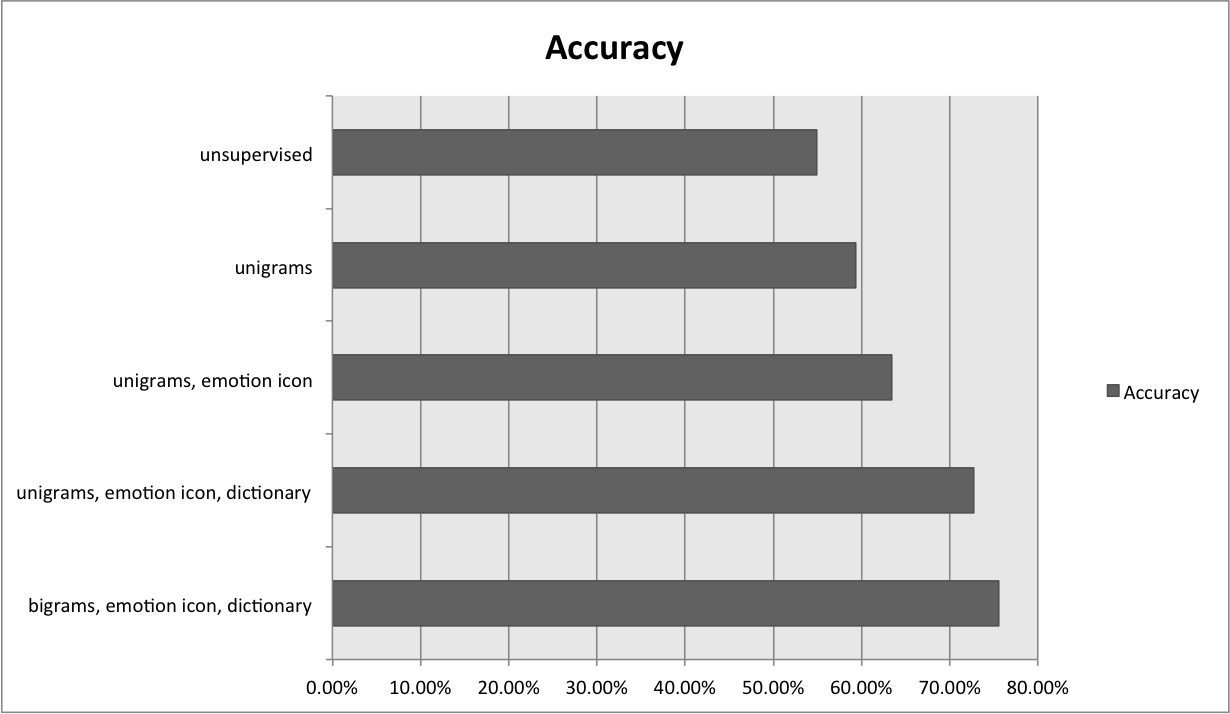
\includegraphics[width=0.9\textwidth]{sentiment_feature.png}
\caption{特征选择}
\label{fig:sentiment_feature}
\end{figure}

我们也尝试了不同的分类模型,包括
\begin{itemize}
\item 朴素贝叶斯
\item 以决策树为基础的AdaBoost
\item 随机森林
\item 线性核SVM
\end{itemize}
测试结果如图\ref{fig:sentiment_model}。线性核SVM表现最好,但朴素贝叶斯也有比较好的性能。

\begin{figure}[!h]
\centering
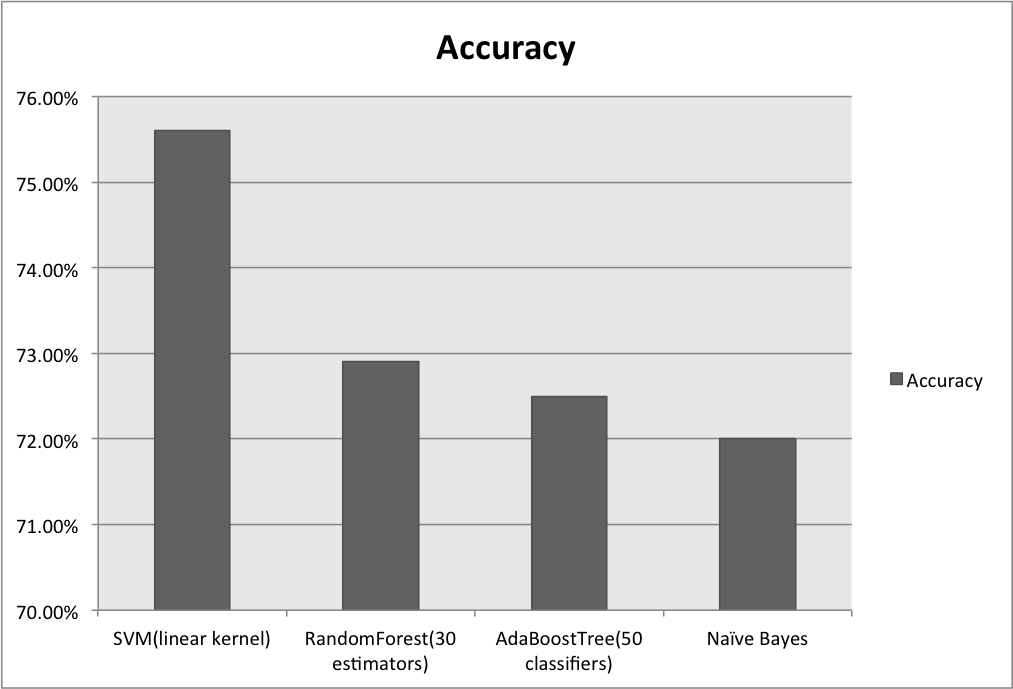
\includegraphics[width=0.8\textwidth]{sentiment_model.png}
\caption{模型选择}
\label{fig:sentiment_model}
\end{figure}

最终达到的75\%的分类精度从数值上看并不是很高,但情感极性的判断有很强的主观性,正面负面和中性并没有很明显的界限。根据之前的研究,人类对情感的判断也只能在79\%的情况下达成一致,因此,一个准确率70\%以上的系统在实际中是可用的。

\subsection{进一步工作}
文档级的情感分类做出了一个假设,即用户在一条微博中只提到一项活动,或者提到多项活动但情感极性是相同的,这在社交媒体短文本的限制下是合理的,在我们的统计中,只有3\%的微博描述多个活动,并且带有相反的情感倾向。但这在实际中并不总是成立。同时,即使同为负面情感,用户的具体情感也可能非常不同,如``疲倦''、``伤心''、``生气''三者代表的情感完全不同,无法用简单的极性表达。Ekman\cite{ekman1992argument}将人类情感分为6中基本情感,``高兴(Happy)'',``激动(Excited)'',``温和(Tender)'',``惊吓(Scared)'',``悲伤(Sad)'',``生气(Angry)''。进一步可以考虑情感的多分类问题。

第二点是,一个活动中会有不同的子方面,如旅游,用户可能会对天气、交通、饮食、住宿等方面分别表达情感。这种aspect-based的细粒度的观点挖掘在商品评论中有比较多的研究,下一步工作中会加以考虑。



